\documentclass[11pt]{report}
\usepackage{cs1200}
\usepackage{graphicx}
\usepackage{float}

\begin{document}
\psHeader{2}{Tue 2026-02-17 (11:59pm)}

Please see the syllabus for the full collaboration and generative AI policy, as well as information on grading, late days, and revisions.

All sources of ideas, including (but not restricted to) any collaborators, AI tools, people outside of the course, websites, ARC tutors, and textbooks other than Hesterberg--Vadhan must be listed on your submitted homework along with a brief description of how they influenced your work. You need not cite core course resources, which are lectures, the Hesterberg--Vadhan textbook, sections, SREs, problem sets and solutions sets from earlier in the semester. If you use any concepts, terminology, or problem-solving approaches not covered in the course material by that point in the semester, you must describe the source of that idea. If you credit an AI tool for a particular idea, then you should also provide a primary source that corroborates it. Github Copilot and similar tools should be turned off when working on programming assignments.

If you did not have any collaborators or external resources, please write 'none.' Please remember to select pages when you submit on Gradescope. A problem set on the border between two letter grades cannot be rounded up if pages are not selected. 
\newline

\textbf{Your name: }Joaquin Gabriel Malachi A. de Castro

\textbf{Collaborators and External Resources: }

\textbf{No. of late days used on previous psets: }0

\textbf{No. of late days used after including this pset: }0

\vspace{1em}

\newpage

\begin{enumerate}
     \item  (designing reductions)
     The purpose of this exercise is to give you practice designing reductions and proving their correctness and runtime.

    Consider the following computational problem:

    \compprob{AreaOfConvexPolygon()}
    {Points $(x_0,y_0),\ldots,(x_{n-1},y_{n-1})$ in the $\R^2$ plane that are the vertices of a convex polygon (in an arbitrary order) whose interior contains the point $(1,1)$.}
    {The area of the polygon formed by the points}

    \begin{enumerate}
        \item \label{part:polar} 
        Show that AreaOfConvexPolygon$\leq_{O(n),n}$ Sorting.  Be sure to analyze both the correctness and runtime of your reduction.

        In this part and the next one, you may assume that a point $(x,y)\in \R^2$ can be converted into polar coordinates $(r,\theta)$ about $(1,1)$ in constant time. 

        You may find the following facts useful and you may use them (as well as other facts from geometry) without proof:
        \begin{itemize}
            \item The polar coordinates $(r,\theta)$ of a point $(x,y)$ about $(1,1)$ are the unique real numbers $r\geq 0$ and $\theta\in [0,2\pi)$ such that $x-1=r\cos \theta$ and $y-1=r\sin \theta$. Or, more geometrically, $r=\sqrt{(x-1)^2+(y-1)^2}$ is the distance of the point from $(1,1)$, and $\theta$ is the angle between the positive $x$-axis and the ray from $(1,1)$ to the point.
            \item The area of a triangle is $A = \sqrt{s(s-a)(s-b)(s-c)}$ where $a, b, c$ are the side lengths of the triangle and $s = \frac{a + b + c}{2}$ (\href{https://en.wikipedia.org/wiki/Heron\%27s_formula}{Heron's Formula}).
        \end{itemize}

        Firstly, given an input $[(x_0,y_0),...,(x_{n-1},y_{n-1})]$, each of these tuples can be converted to polar in $O(1)$ + $O(1)$ time.
        Since there are n elements, this conversion step takes $O(n)$ time.
        Of note, we can choose to do this in such a way that in the resulting tuple, the first element of each or the key is the angle while the second is the radial component.
        This is because we will sort with the angles as our key. 

        Now we can make one call to the oracle that solves Sorting, sorting our resulting list of points by their angles.

        This gives us a list of adjacent points.
        Pairing up consecutive points along with the point $(1,1)$ partitions the polygon into triangles, whose areas when added up gives the area of the whole polygon.

        Specifically, $\forall i \in range(n),$ our side lengths are
        
        $a = r_i$

        $b=r_{i+1}$

        $c=\sqrt{r_i^2+r_{i+1}^2+2 r_i r_{i+1} \cos(\theta_{i+1} - \theta_{i})}$

        We can then plug in these side lengths to heron's formula to solve for the area of each triangle.

        Assuming these take O(1) time to compute, finding the area of all of these triangles takes O(n) time.

        Summing each of these also takes time O(n) for n triangles to sum.

        Thus in total, assuming that an oracle call to Solving takes O(1) time, T(n) for this reduction is O(n). We only make one call to sorting (q=1), and each call to sorting takes as an input an array of size n.

        These gives in reduction notation $O(n),n$


        
        \item Deduce that AreaOfConvexPolygon can be solved in time $O(n\log n)$.
        We know that given a reduction $T(n),h(n),q(n)$, AreaOfConvexPolygon takes
        $T(n) + q(n)*f(h(n))$ where $f$ is the runtime of sorting.
        Plugging in our known values gives a runtime of
        $O(n) + O(n\log{n}) = O(n\log{n})$
        
        \item (*challenge; extra credit; optional\footnote{This problem is meant to be done based on your enjoyment/interest and only if you have time. It won't make a difference between N, L, R-, and R grades (meaning it will only impact whether an R gets increased to an R+), and course staff will deprioritize questions about this problem at office hours and on Ed.})  Come up with a way to avoid conversion to polar coordinates and any other trigonometric functions in solving AreaOfConvexPolygon in time $O(n\log n)$.  Specifically, design an $O(n)$-time reduction that makes $O(1)$ calls to a Sorting oracle on arrays of length at most $n$, using only arithmetic operations $+$, $-$, $\times$, $\div$, and $\sqrt{\hspace{1em}}$, along with comparators like $<$ and $==$.  (Hint: first partition the input points according to which quadrant they belong in, and consider the slope of the line from a vertex (x,y) to the origin.) \label{part:nopolar}
        
\end{enumerate}
    
    Similar techniques to what you are using in this problem are used in algorithms for other important geometric problems, like finding the Convex Hull of a set of points, which has applications in graphics and machine learning.




    \item (composition of reductions) 
 The purpose of this exercise is to give you practice in working with the abstract definition of reductions. 
    
    Let $\Pi, \Gamma, \Lambda$ be computational problems, and suppose that $\Pi\leq_{T_1(n),q_1(n)\otimes h_1(n)} \Gamma$ and \\ $\Gamma \leq_{T_2(n),q_2(n)\otimes h_2(n)} \Lambda$, for non-decreasing functions $T_1,T_2,q_1,q_2,h_1,h_2$.  Determine functions $T_3,q_3,h_3$ in terms of $T_1,T_2,q_1,q_2,h_1,h_2$ such that 
    $$\Pi \leq_{O(T_3(n)),q_3(n)\otimes h_3(n)} \Lambda,$$
    and justify your answers. You do not need to prove the correctness of the reduction from $\Pi$ to $\Lambda$. Just justify the functions $T_3$, $q_3$ and $h_3$. (Hint: you can take $h_3(n)=h_2(h_1(n))$.)

    Given that $\Gamma$ has a runtime of $T_2$ when assuming that calls to an oracle for $\Lambda$ is O(1),
    how long does $\Pi$ take under the same assumption?
    Well, this would just

    $T_3(n) = T_1(n) + q_1(n)*T_2(h(n))$

    Now to find q and h I find an explicit formula without yet assuming that oracle calls to gamma take O(1) and instead call the runtime of $\Gamma$ $g$

    I wrote a draft of my solution on a blackboard and just asked ChatGPT to convert it to LaTeX for me: https://chatgpt.com/share/e/6995276f-5d18-8000-a95f-7d4b5431d140

\[
\text{How long does } \Pi \text{ take if } \Gamma = O(f(n))?
\]

\[
\Rightarrow \; T_1(n) + q_1(n) f(h_1(n))
\]

\[
\text{How long does } \Gamma \text{ take given } \Lambda = O(g(n))?
\]

\[
\Rightarrow \; f(n) = T_2(n) + q_2(n) g(h_2(n))
\]

\[
\Pi \text{ takes }
T_1(n) + q_1(n)\Big[ T_2(h_1(n)) + q_2(h_1(n)) g(h_2(h_1(n))) \Big]
\]

\[
\text{If } g(n)=1,\text{ this gives a runtime for }  \Pi :
\]

\[
T_1(n)
+
q_1(n)\Big[
T_2(h_1(n)) + q_2(h_1(n))
\Big]
\]

\[
\text{The coefficient of } g \text{ gives us \# of oracle calls to } g
\]

\[
q_3(n) = q_1(n)\, q_2(h_1(n))
\]

\[
\text{The argument in } g \text{ gives } h_3
\]

\[
h_3(n) = h_2(h_1(n))
\]



    \newpage

    
    \item (augmented binary search trees)
    The purpose of this problem is to give you experience reasoning about correctness and efficiency of dynamic data-structure operations, on variants of binary-search trees. You may assume that all keys are distinct.
    
    Specifically, we will work with {\em selection data structures}.
    We have seen how binary search trees can support $\minq$ queries in time $O(h)$, where $h$ is the height of the tree.  A generalization is {\em selection} queries, where given a natural number $q$, we want to return the $q$'th smallest element of the set.  So $\texttt{DS.select(0)}$ should return the key-value pair with the minimum key among those stored by the data structure $\texttt{DS}$, $\texttt{DS.select(1)}$ should return the one with the second-smallest key, $\texttt{DS.select(n-1)}$ should return the one with the maximum key if the set is of size $n$, and $\texttt{DS.select((n-1)/2)}$ should return the median element if $n$ is odd.
    
    It is known that if we {\em augment} binary search trees by adding to each node $v$ the size of the subtree rooted at $v$, then $\selectq$ queries can be answered in time $O(h)$.\footnote{Note that the Roughgarden text uses a different indexing than us for the inputs to $\selectq$. For Roughgarden, the minimum key is selected by $\selectq(1)$, whereas for us it is selected by $\selectq(0)$.}

    
    \begin{enumerate}
        \item In the Github repository, we have given you a Python implementation of size-augmented BSTs supporting search, insertion, and selection, and with a stub for \texttt{rotate}. One of the implemented functions (\texttt{search}, \texttt{insert}, or \texttt{select}) has a correctness error, another one is too slow (running in time that's (at least) linear in the number of nodes of the tree rather than linear in the height of tree), and the third is correct. 
        Identify and correct these errors. You should provide a text explanation of the errors and your corrections, as well as implement the corrections in Python.    


        Answer:
        
        Search()

        Search correctly goes through the tree in logarithmic time by excluding the left or right children from the search at each rank, thus not having to iterate over all n nodes.

        Select()
        
        I was testing the function on a BST representation of [1,2,3,5,7,6,9]

        I found that when Selecting on sufficiently large of an index, Select fails

        I realized that this was because we were passing the same big index even to the smaller right child tree.

        Consider Select(5), even if after we move to the right from 5 to its right child 7, the algorithm still tells it to look for the element with 5 smaller elements\dots

        even though we have already found nodes outside of this right tree that are smaller than all of it.

        Specifically, everytime we move to the right, the size of the left tree and the root node we are coming from are all smaller than any node we will find in the right tree.

        So we only need to find an element with $ind - left\_size - 1$ elements in the right tree smaller than it.
        
        This is fixed in my implementation of the function where I pass this updated index to the recursion when moving to the right.

        After testing on the same BST, all seems to be in order (quite literally).

        Describe (in pseudocode or pictures) how to extend \texttt{rotate} to size-augmented BSTs, and argue that your extension maintains the runtime $O(1)$. Prove that your new rotation operation preserves the invariant of correct size-augmentations. (That is, if every node's size attribute had the correct subtree size before the operation, then the same is true after the operation.)
        
        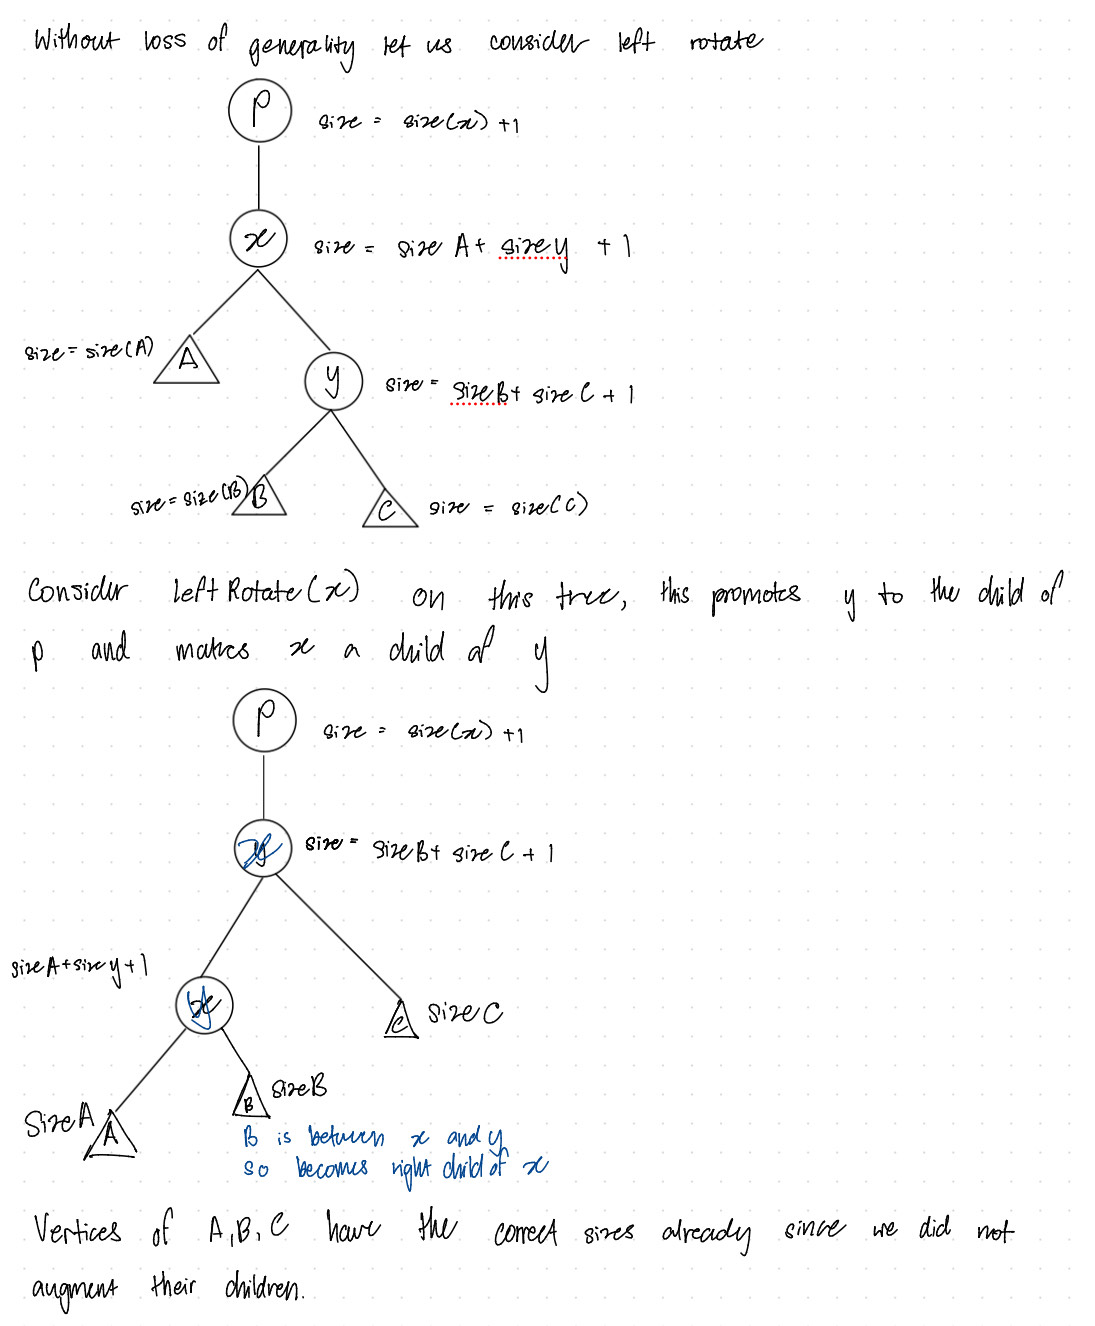
\includegraphics[width=\textwidth, height=\textheight, keepaspectratio]{3A1.jpeg}
        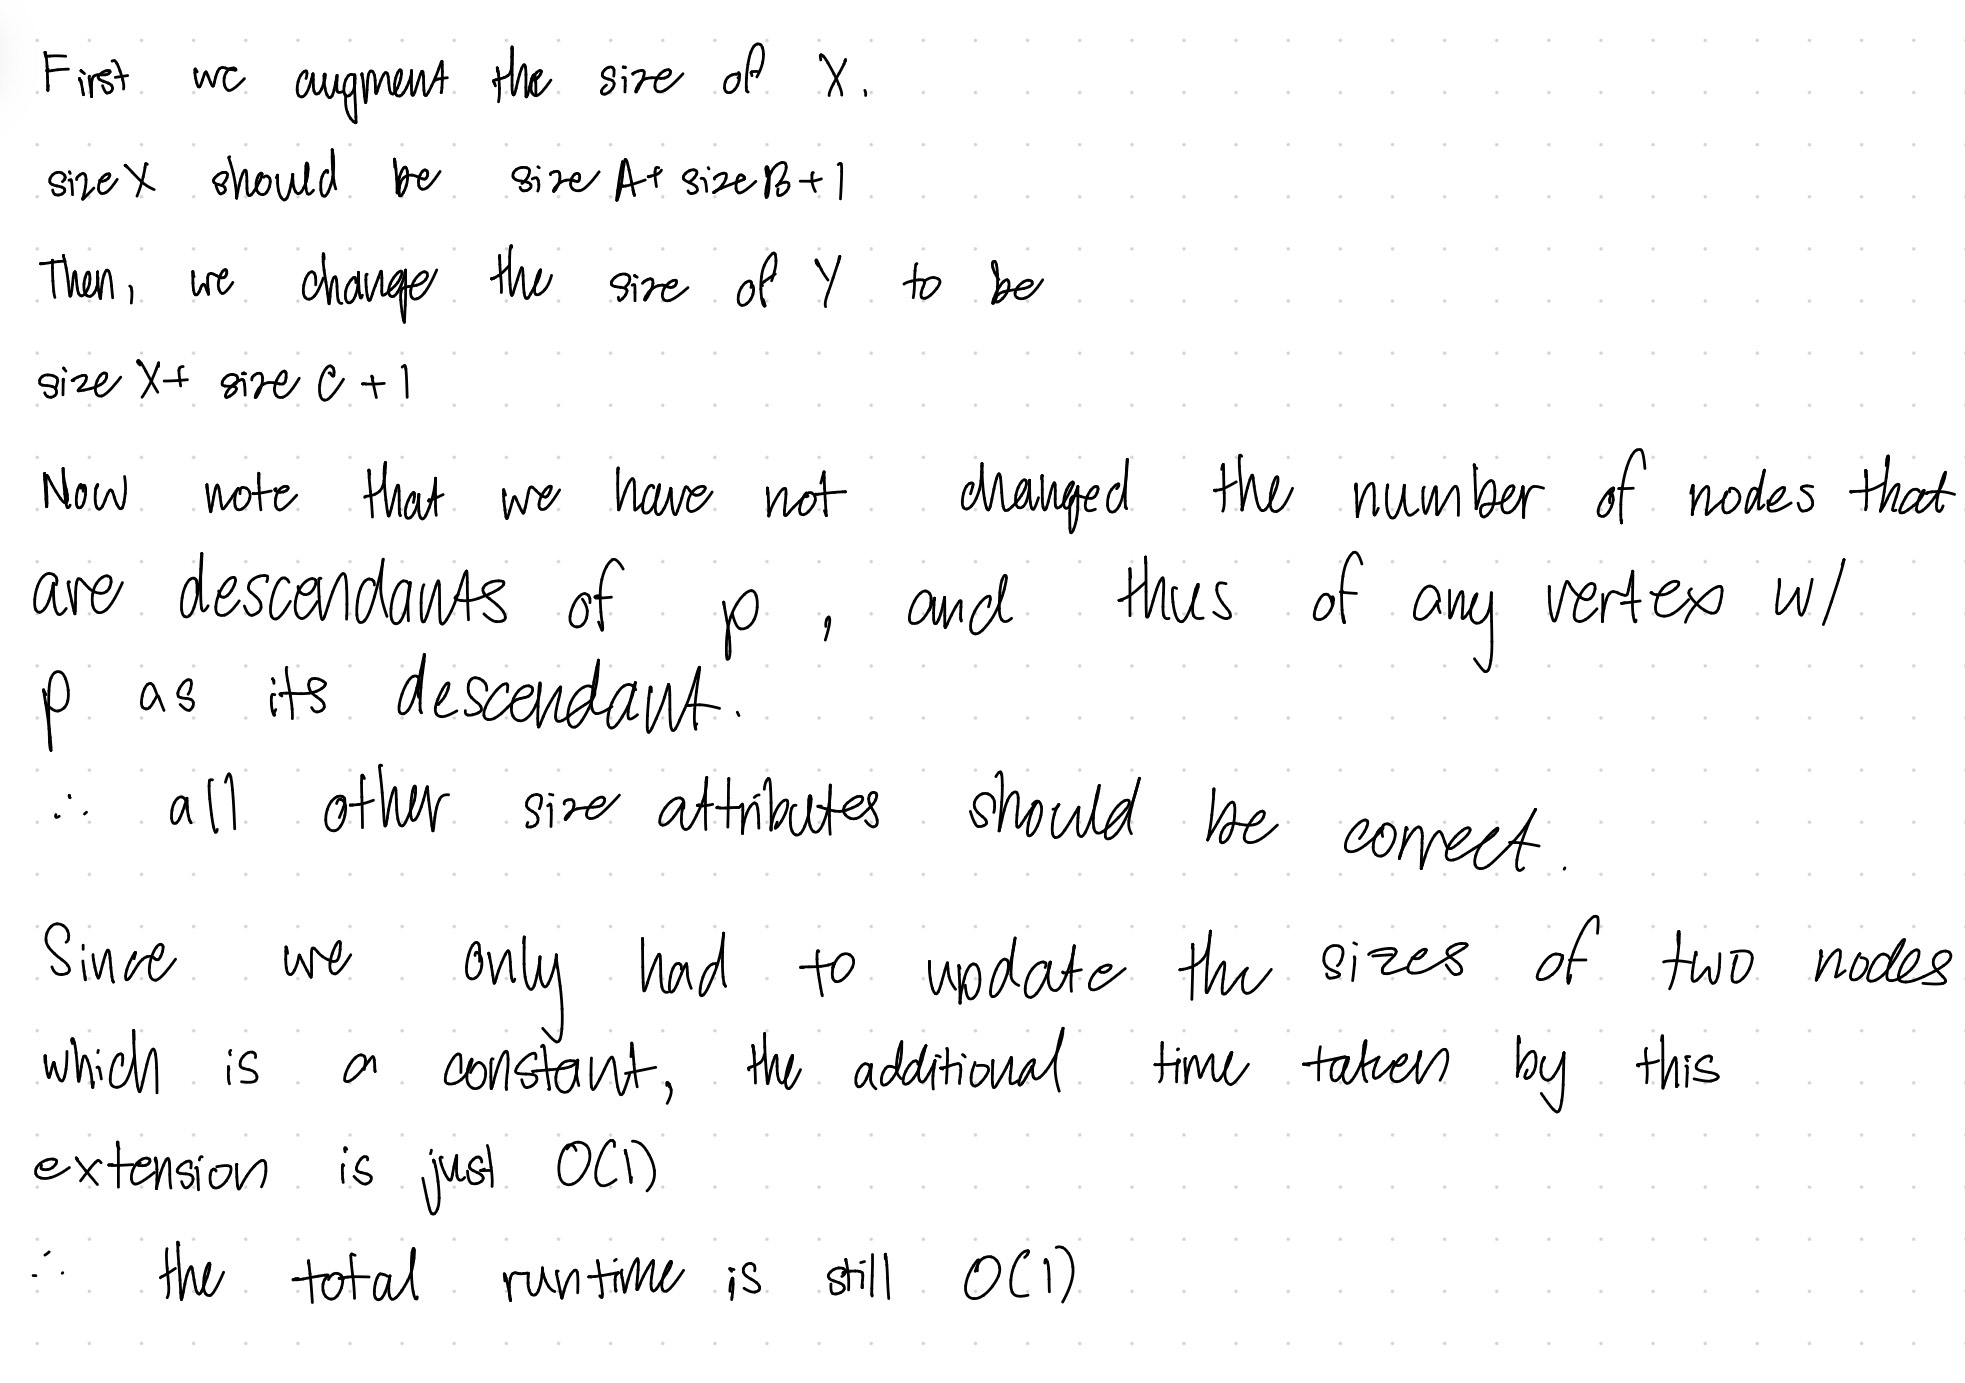
\includegraphics[width=\textwidth, height=\textheight, keepaspectratio]{3A2.jpeg}

        \item Implement \texttt{rotate} in size-augmented BSTs in Python in the stub we have given you.
        In addition to doing this, I also added a $printb()$ function which helped me check my work by printing out an outline of the tree. I also tested my implementation on an example tree shown in the ipynb notebook file.
    
    \end{enumerate}
    
    \emph{Food for thought (do read - it's an important take-away from this problem):} This problem concerns size-augmented binary search trees. In lecture, we discussed AVL trees, which are balanced binary search trees where every vertex contains an additional \textit{height} attribute containing the length of the longest path from the vertex to a leaf (height-augmented). Additionally, every pair of siblings in the tree have heights differing by at most 1, so the tree is height-balanced. Note that if we augment a binary search tree both by size (as in the above problem) and by height (and use it to maintain the AVL property), then we create a dynamic data structure able to perform \texttt{search}, \texttt{insert}, and \texttt{select} all in time $O(\log n)$. 


\item (reflection) We aim for cs1200 to be a collaborative learning community. Describe two concrete ways in which you have supported, or will try to support, your classmates' learning in the course.  Be specific, connecting your answer to the structure of cs1200. Good answers are at least 6-8 sentences in length.

\textit{Note: As with the previous psets, you may include your answer in your PDF submission, but the answer should ultimately go into a separate Gradescope submission form.}



\item Once you're done with this problem set, please fill out \href{https://forms.gle/wwedZAhPduqzHQ9d8}{this survey} so that we can gather students' thoughts on the problem set, and the class in general. It's not required, but we really appreciate all responses!

\end{enumerate}

\end{document}
